\chapter{DTLS}

\section{What is it ?}

DTLS (Datagram Transport Layer Security) is a protocol designed to communicate securely over UDP. It was first presented in \cite{modadugu2004design} by Mogadugu and Rescorla as an adaptation of TLS for delay sensitive applications. The objective was to be as close as possible from TLS while being as secure over an unreliable transport protocol. As TLS, this protocol operates at level 5 in the OSI model. It means you don't need to modify your kernel to use it.

The current version of this protocol is currently DTLS 1.2 described in RFC6347 \cite{rfc6347}. Our work is based on this version because no effort concerning a possible version 3 has been noticed recently. We may expect such a version will come after the discussions on TLS 1.3 that are taking place as we write these lines. For now, the suggested modifications have no impact on our current design as we explain in Section \ref{sec:} \todo{insert reference}.

Even if this protocol is standardized for some years, rare are the important applications using it. In the open source world, openVPN has planned to use it when UDP is used. Unfortunately, it seems not to be a top priority and they are still using a homemade protocol to do TLS over UDP.

We have found a simpler VPN application using DTLS v1 called Campagnol. More details on how we modified it and integrate our solution are provided in Section \ref{sec:}\todo{add reference}.

\section{How does it work ?}

In this section we present an overview of how DTLS works. We begin by a recall of TLS goals and principles since it is strongly related. Then, we go through the major differences between these two protocols. Finally, we list the steps in a typical connection and present the different messages involved. 

\subsection{TLS}

TLS is a protocol designed to provide a secure connection over reliable transport. It takes place between a server and a client. 

Once the channel is established :

\begin{itemize}
\item The client has authenticated the server (i.e. the server is really the one he pretends to be).
\item All messages can only be read by the other host (an eavesdropping is possible but the clear text cannot be obtained)
\item The packets cannot be replayed or modified on the line without the host noticing.
\end{itemize}

To achieve the two last points, cryptography is used between the two hosts and the packets are also signed. TLS authentication typically uses digital signature based on public key together with a Certification Authority. During the handshake, the two hosts are negotiating which version of protocol will be used together with algorithms to encrypt and sign the future messages. A traditional handshake with no authentication from the client\footnote{This is only optional and will simply add some more messages for the server to be able to verify the client identity.} and RSA as cipher suite is depicted in figure \ref{fig:tls_handshake}.


\begin{figure}[!ht]
\centering
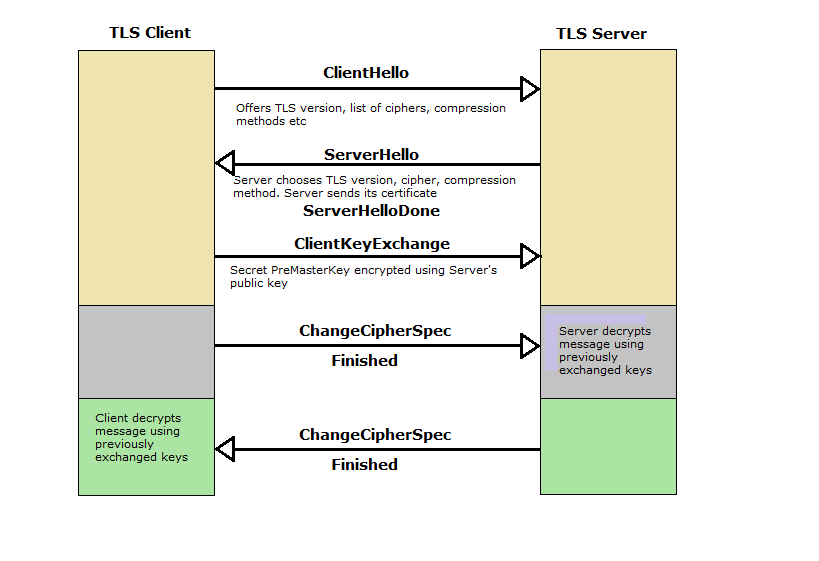
\includegraphics[width=0.9\textwidth]{images/tls-handshake.png}
\caption{Typical TLS handshake}
\label{fig:tls_handshake}
\end{figure}

In the first phase, the client will give his version together with a list of algorithms for encryption and compression. The server will then choose among the ones proposed : the version, cipher suite and compression method to be used for the rest of the communication. In addition, the server may provide a session ID which can be used later for session resumption.

The server also provides his certificate to the client. It contains enough information for the latter to be able to verify the server identity. When the server sends his 'ServerHelloDone' message, he indicates the negotiation is now finished on his side.

The next step comes with the client computing a \textit{PreMasterKey}. This key is sent securely because it is encrypted with the server public key. Therefore only the possessor of the private key (the server) can retrieve the content of the message. From this key and a random number exchanged during the clientHello/serverHello messages, the master key is computed by each host.

The 'changeCipherSpec' message is sent by a host to the other to explicitly say that the following messages will be encrypted and signed with the parameters negotiated. Then the 'finished' message conclude the handshake and contains a MAC of all previous messages. If the receiving host is able to decrypt the message and reconstruct the MAC, then everything was done correctly and the connection can continue with keys deduced from the master key.

All messages following the handshake (containing application data) will be encrypted with symmetric cryptography using the keys deduced from the master key for this particular session. Note that the knowledge of one of the ephemeral key does not allow an attacker to retrieve the long-term keys used for the handshake.

To avoid packet to be replayed by an attacker and therefore disturb the normal communication, TLS signs packet with a sequence number associate with it. The sequence number is incremented for every packet sent. Thus, two counts must be considered : one for packets sent and the other for packets received. Thanks to a reliable transport protocol, these counts must never be transmitted explicitly because each host can compute them. As a conclusion, if an attacker try to replay packets, they will simply be rejected because the signature will not match with the most recent sequence number.



\subsection{Differences from TLS}


\subsection{DTLS Handshake}

\section{Choice of Library}

Our starting point with DTLS was to use an existing library. Multiple libraries implement the latest version \footnote{\url{https://en.wikipedia.org/wiki/Datagram_Transport_Layer_Security\#Implementations}}, but we chose wolfSSL (previously CyaSSL) to handle this part.

The choice was done following multiple criteria :

\begin{itemize}
\item Clarity of code
\item Documentation
\item Existing examples
\item Library size
\end{itemize}

Unlike OpenSSL, wolfSSl contains a reduced number of files to handle SSL/TLS and DTLS. The objective of this library is to be as light as possible to allow integration in embedded systems. As stated in their official website \footnote{\url{http://www.yassl.com/yaSSL/Home.html}}, the library is up to 20 times smaller than OpenSSL. Since it is also a commercial product used for private solutions, it can be a gage of quality. 

A documentation and working examples are provided to help people using it.
